\documentclass{beamer}
\usepackage[latin1]{inputenc}
\usepackage{movie15}
\usepackage{comment}
\usepackage{graphicx}
\usepackage{subfig}
\usetheme{Ilmenau} %Warsaw,  Antibes, PaloAlto, Malmoe
\usecolortheme{default} %wolverine=geel/orange, beaver=darkred/blue, default=blue



\title[Item Reponse Theory in Intelligent Tutoring Systems]{Parameter invariance in IRT based models} %eerste is titel van hele presentatie
\author{Lieuwe Rekker}
\institute{University of Amsterdam}
\date{December 18, 2014}



\begin{document}


\frame{\titlepage} 



\frame{\frametitle{Table of contents}\tableofcontents} 


%%%%%%%%%%%%%%%%%%%%%%%%%%%%%%%%%%%%%%
%Algemene deel
%%%%%%%%%%%%%%%%%%%%%%%%%%%%%%%%%%%%%%
\section{Context}
\subsection{Intelligent Tutor Systems \& Learner Models}
\frame{\frametitle{Intelligent Tutor System}

	\begin{itemize}
		\item Computer program for students to practice
		\item Replacement for pen \& paper questions
		\begin{itemize}
			\pause \item Direct and personalized feedback
			\item Adjusted curriculum
		\end{itemize}
		\pause \item Educational datasets:
		\begin{itemize}
			\pause \item Question = datapoint: student,item and answer
			\pause \item Item to knowledge component mapping
		\end{itemize}
	\end{itemize}
}

%%%%%%%%%%%%%%%%%%%%%%%%%%%%%%%%%%%%%%%

\frame{\frametitle{Learner Model}
	\begin{itemize}
		\item Question $\Rightarrow$ answer prediction
		\pause \item Two methods of assessing 
		\begin{itemize}
			\pause \item Prediction accuracy
			\item External measures (e.g. post-test)
		\end{itemize}
		\pause \item Item Response Theory uses an additional method 
	\end{itemize}
}

\frame{\frametitle{Item Response Theory}
	\begin{itemize}
		\item Standardized testing
		\item Works similarly to learner model (except no learning)
		\item Assessing parameters
		\begin{itemize}
			\pause \item Cornerstone: invariability of parameter values
		\end{itemize}
	\end{itemize}
}

\subsection{Models}
\frame{\frametitle{Invariable parameters}
\begin{center}
\begin{figure}
  
    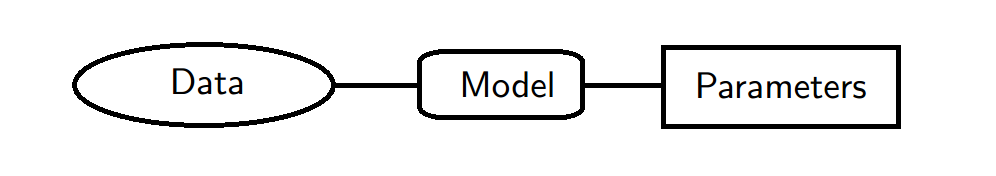
\includegraphics[width=3in]{images/summary.png}
  
\end{figure} 

\begin{figure}
  
    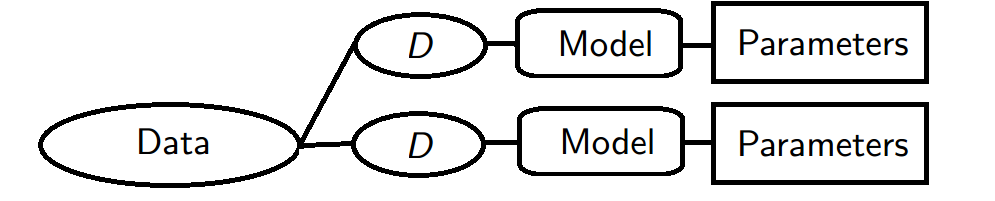
\includegraphics[width=3in]{images/summary2.png}
  
\end{figure}
\end{center}
}


\subsection{Models}
\frame{\frametitle{Logistic Function}
\begin{center}
$ \sigma(x) = \frac{1}{1+e^{-x}}$

\begin{figure}
  
    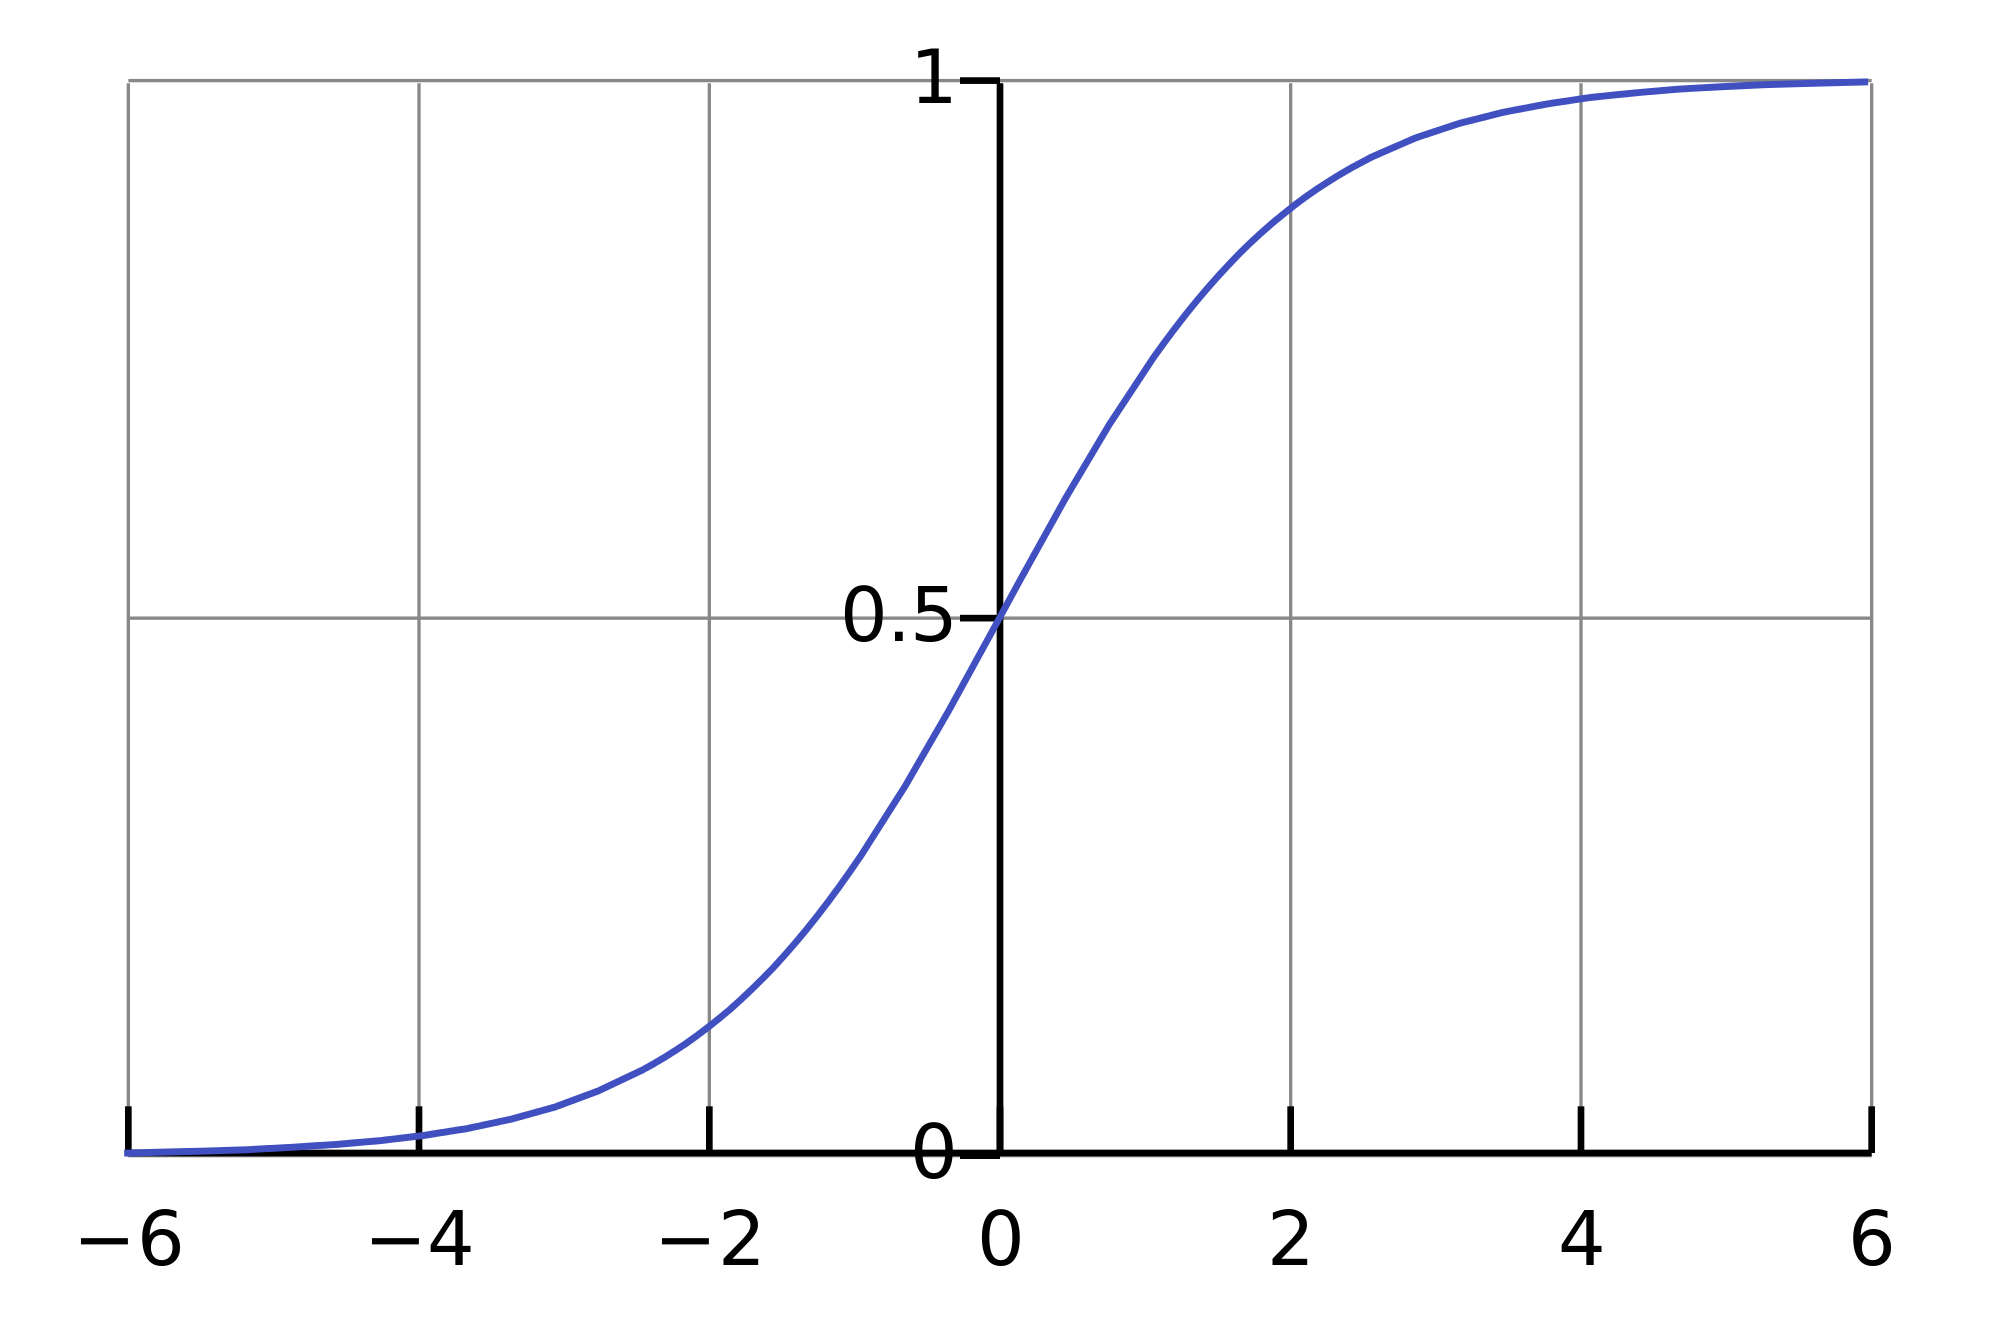
\includegraphics[width=3in]{images/sigmoid.png}
  
\end{figure} 
\end{center}
}

\frame{\frametitle{IRT-based Learner Models}
	\begin{itemize}
		\item Learning Factor Analysis Model (LFA)
		\begin{itemize}
			\item $P(s,i) = \sigma(\theta_{s,0} + \sum_{c \in KC_{i}}(\gamma_{c} t_{s,c} - \beta_{c}))$
		\end{itemize}
		\pause \item Performance Factor Analysis Model+ (PFA+)
		\begin{itemize}
			\item $P(s,i) = \sigma(\theta_{s,0} + \sum_{c \in KC_{i}} (\gamma_{c} g_{s,c} + \rho_{c} f_{s,c} - \beta_{c}))$
		\end{itemize}
		\pause \item Multidimensional extended IRT Model (meIRT)
		\begin{itemize}
			\item $P(s,i) = \sigma(\sum_{c \in KC_{i}} (\alpha_{c}(\frac{\theta_{s,0}}{|KC_{i}|} + \eta_{s} t_{s,c}) - \beta_{c}))$
		\end{itemize}
	\end{itemize}
}

%%%%%%%%%%%%%%%%%%%%%%%%%%%%%%%%%%%%%%%


\frame{\frametitle{Fitting Parameters}
	\begin{itemize}
		\item Maximize Likelihood of the data
		\begin{itemize}
			\pause \item $L(D)=\prod_{d \in D} P_{d}^{t_d}  (1- P_{d})^{1-t_d}$
		\end{itemize}
		\pause \item Logistic Regression for LFA and PFA
		\pause \item Iterative Logistic Regression for meIRT
		\begin{itemize}
			\pause \item Keep student parameters fixed
			\pause \item Keep KC parameters fixed
		\end{itemize}
	\end{itemize}
}

\section{Research Question}
\frame{\frametitle{Research Question}
	\begin{itemize}
		\item IRT-based models without IRT methodology: little consideration for parameters.
		\pause \item To what extent are the knowledge component (KC) parameters of IRT based learner models invariant?
		\begin{itemize}
			\pause \item To what extent are the rank-orderings of the KC parameter-types invariant?
			\pause \item What is the standard deviation of the KC parameter values over subsets of the data?
			\pause \item What is the influence of the amount of data on invariability?
			\pause \item To what extent is invariability of parameters expected given the stochasticity of the model?
		\end{itemize}
	\end{itemize}
}
\section{Methods}
\subsection{Approach}
\frame{\frametitle{Splitting Data}
	\begin{itemize}
		\item Data is split on students
		\begin{itemize}
			\pause \item Data which could naturally occur in an ITS
			\pause \item Practical
		\end{itemize}
		\pause \item Split into 6,8,12,16 and 32 parts
	\end{itemize}
}

\subsection{Measures}
\frame{\frametitle{Rank Order Correlation}
	\begin{itemize}
		\item Kendall's Tau
		\begin{itemize}
			\pause \item $\tau=\frac{S-D}{\frac{1}{2} n (n-1)}$
		\end{itemize}
		\pause \item $\frac{\tau+1}{2}$ of the orderings are the same
	\end{itemize}	
}

\frame{\frametitle{Inherent Variability}
	\begin{itemize}
		\item Probabilistic models
		\pause \item Generating answers $\Rightarrow$ different datasets $\Rightarrow$ different parameters
		\pause \item Generate 10 answersets $\Rightarrow$ fit models $\Rightarrow$ standard deviation over 10 models
		\pause \item Average $\tau$ over every combination of models
	\end{itemize}
}

\frame{\frametitle{Inherent Variability in the Experiment}

\begin{figure}
  \begin{center}
    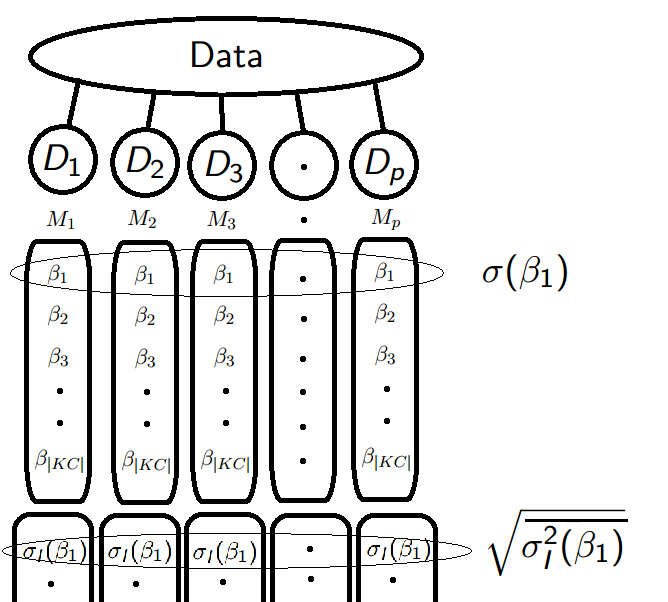
\includegraphics[width=2.5in]{images/uitleg2.png}
  \end{center}
\end{figure} 
}

\frame{\frametitle{Datasets}

\begin{tabular}{| l | l | l | l |}
    \hline
    Dataset & \# questions & \# KCs\tiny{(removed)} &\# students\tiny{(removed)}\\ \hline
    Bridge & 1,814,398 & 455\tiny{(34)} & 1129\tiny{(17)}  \\ \hline
    Algebra & 585,557 & 104\tiny{(6)} & 564\tiny{(10)}\\ \hline
    Assistment & 110,842  & 106\tiny{(0)} & 425\tiny{(20)}\\
    \hline
\end{tabular}
}

\section{Results}
\frame{\frametitle{Rank order invariability}
\begin{figure}
\begin{center}
  \subfloat{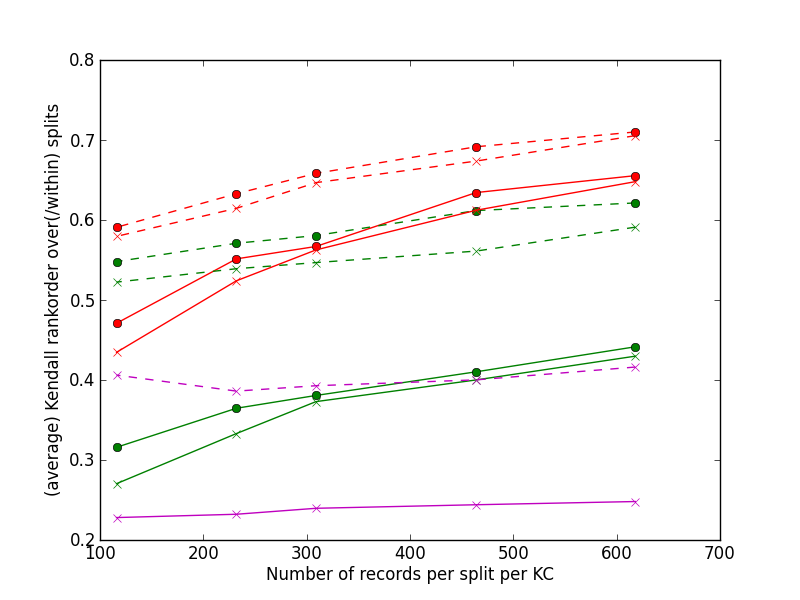
\includegraphics[width=3in]{images/bridgeallmodranksKC.png}}                
  \subfloat{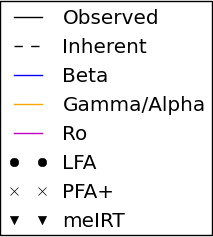
\includegraphics[width=0.5in]{images/legend.png}}
\end{center}
\end{figure}
}

\frame{\frametitle{Displaying Average Standard Deviation per Parameter-Type}
\begin{figure}
  \begin{center}
    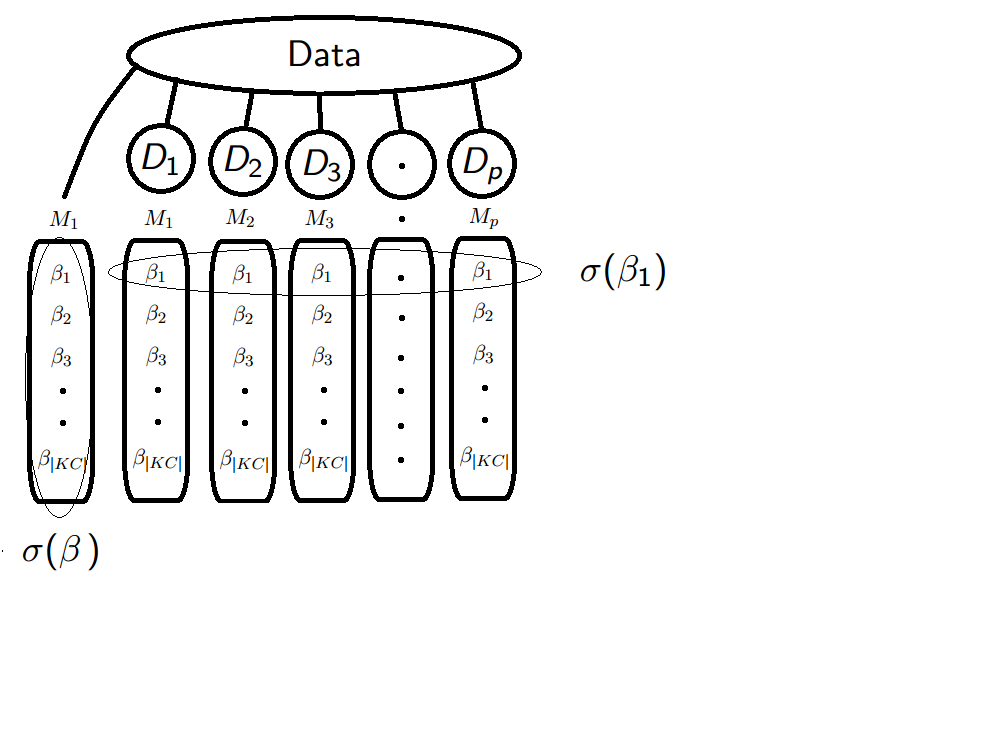
\includegraphics[width=3.5in]{images/uitleg3.png}
  \end{center}
\end{figure} 
}


\frame{\frametitle{Average Standard Deviation per Parameter-Type}
\begin{figure}
\begin{center}
  \subfloat{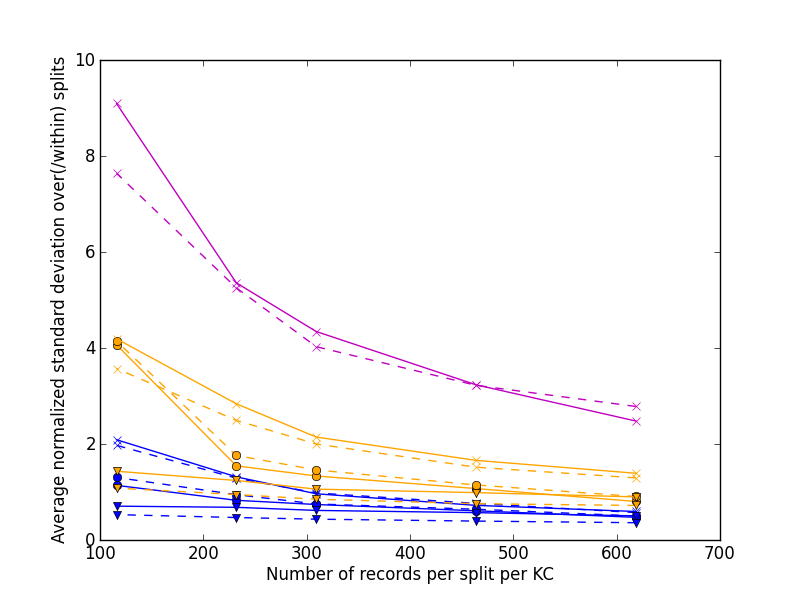
\includegraphics[width=3in]{images/bridgeallmodsdsKC.png}}                
  \subfloat{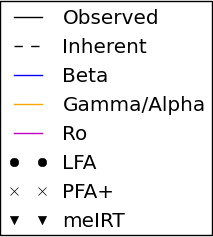
\includegraphics[width=0.5in]{images/legend.png}}
\end{center}
\end{figure}
}


\frame{\frametitle{Standard Deviation within Parameter-Types}
\begin{figure}
\begin{center}
  \subfloat{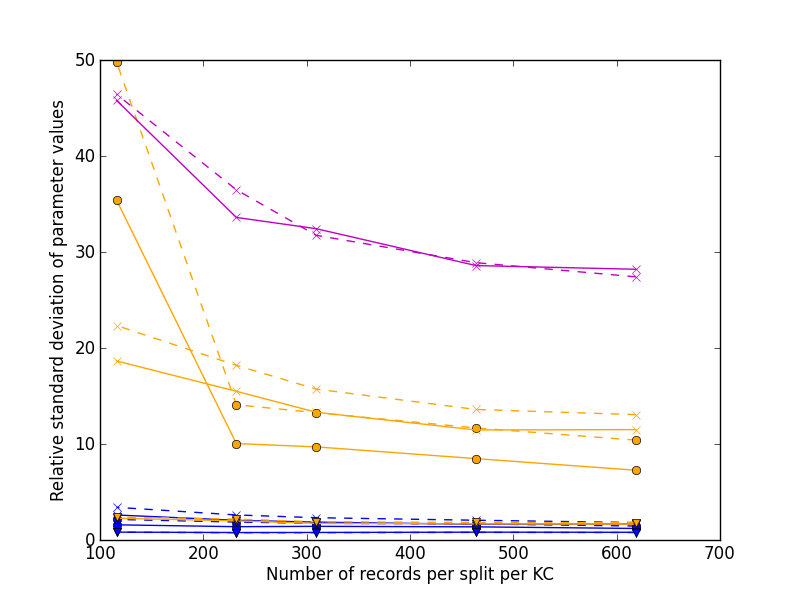
\includegraphics[width=3in]{images/bridgeallmodsparvar.png}}                
  \subfloat{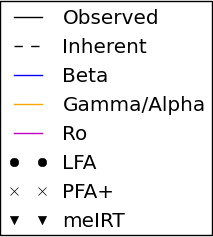
\includegraphics[width=0.5in]{images/legend.png}}
\end{center}
\end{figure}
}

\frame{\frametitle{Standard Deviation within Parameter-Types: Detail}
\begin{figure}
\begin{center}
  \subfloat{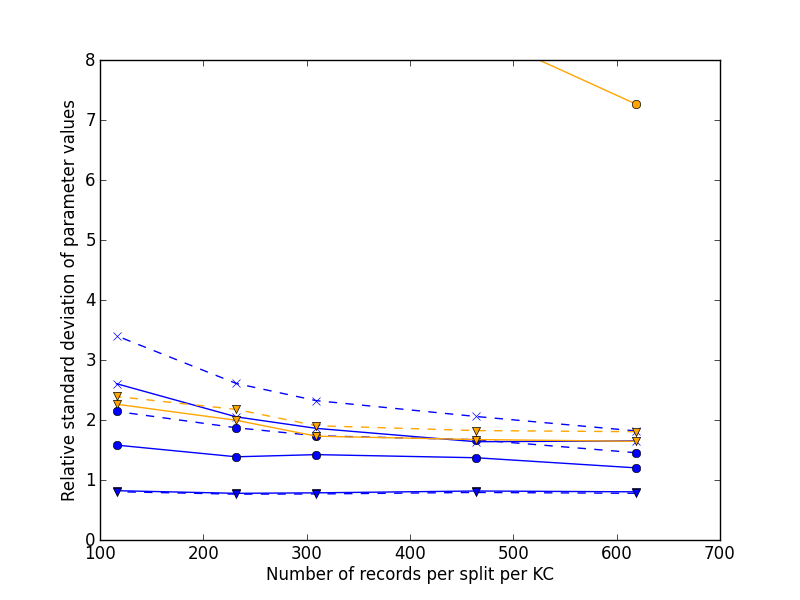
\includegraphics[width=3in]{images/bridgeallmodsparvarz.png}}                
  \subfloat{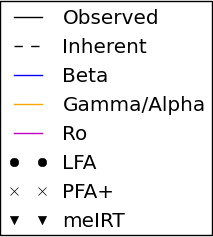
\includegraphics[width=0.5in]{images/legend.png}}
\end{center}
\end{figure}
}

\section{Conclusion \& Discussion}

\begin{comment}
\frame{\frametitle{Results Summary}
	\begin{itemize}
		\item Rank Order Invariance
		\begin{itemize}
			\item Only $\beta$ parameters score well
			\item $\tau$ over generated data provides a good upper bound
			\item As data increases $\tau$ decreases
		\end{itemize}
		\pause \item Average Parameter Standard Deviation
		\begin{itemize}
			\item Parameter sizes increase as amount of data decreases (especially for LFA and PFA+ models)
			\item Parameter sizes of generated data often $\>$ parameter sizes of observed data
		\end{itemize}
	\end{itemize}
}
\end{comment}


\frame{\frametitle{Conclusion}
	\begin{itemize}
		\item LFA and PFA+ on a whole are poor models to use
		\begin{itemize}			
			\item Poor learning parameter rank-order invariance
			\item Parameter sizes decrease as amount of data increases
		\end{itemize}
		\pause \item meIRT also poor model to use
		\begin{itemize}	
			\item Poor $\alpha$ parameter rank-order invariance
			\item Less problems with changing parameter sizes
		\end{itemize}
		\pause \item $\tau$ over generated data provides a good upper bound
	\end{itemize}
}

\frame{\frametitle{Discussion}
	\begin{itemize}
		\item Limitations
		\begin{itemize}			
			\item Look at individual parameters
			\item Interpretable metric: average correct at start and at end
		\end{itemize}
		\pause \item Further research
		\begin{itemize}			
			\item Use more data
			\item Fix parameters for students/knowledge components 
		\end{itemize}
		
	\end{itemize}
}

\frame{\frametitle{Thank you}
\begin{center}
Thank you for your attention
\end{center}
}
\end{document}

%
%\subsection{joining picture and lists} 
%
%\frame{
%\frametitle{pictures and lists in beamer class}
%\begin{columns}
%\begin{column}{5cm}
%\begin{itemize}
%\item<1$\Rightarrow$ subject 1
%\item<3$\Rightarrow$ subject 2
%\item<5$\Rightarrow$ subject 3
%\end{itemize}
%\vspace{3cm} 
%\end{column}


%\begin{column}{5cm}
%\begin{overprint}
%\includegraphics<2>{PIC1}
%\includegraphics<4>{PIC2}
%\includegraphics<6>{PIC3}
%\end{overprint}
%\end{column}
%\end{columns}}
%
%%%%%%%%%%%%%%%%%%%%%%%%%%%%%%%%%%%%%%%%


